% Anisoptera-Zygoptera are switched in the code output box notes on p.18 
% Fix bandwith error on density plots   

\chapter{$t$ tests and $F$ tests}
\label{ch:t_F_tests}

Aims of this chapter\footnote{Here you work with the script file {\tt t\_F\_tests.R}}:
\begin{compactitem}
	\item Using $t$ tests to look at differences between means
	\item Using $F$ tests to compare the variance of two samples
	\item Using non-parametric tests for differences
\end{compactitem}

In the last chapter, we looked at the genome size and morphology of 
species of dragonflies and damselflies (Odonates: Anisoptera and 
Zygoptera). Box and whisker plots and density plots both show that the 
two groups have rather different genome size and morphology. We can use 
$t$ tests to test whether the means of the variables of the two groups 
are different and we can use the $F$ test to check whether they have 
the same variance.

In this chapter, we will continue to practise building scripts and 
creating your own R code, so we will start from an empty script file. 
Use this script to store the code you run in this practical session and 
add notes to keep a record of what each bit is doing:

\begin{compactitem}[$\quad\star$]
	\item Open R and change to the {\tt Code} directory.
	\item If you have misplaced the data then it is on Blackboard / 
	Bitbucket, so download it again.
	\item Create a new blank script called {\tt ttests.R} and save it to 
	the working directory.
	\item Put a comment at the top (using \#) to describe the script 
	and.
	\item For the rest of this session, type your code into this script, 
	adding comments and then run them in R using Ctrl+R. If you make 
	mistakes, correct the script and run the code again. This way you 
	will end up with a complete neat version of the commands for your 
	analysis. 
	\item Add code to your script to load the genome size data into R, 
	assigning the object name {\tt genome} and use {\tt str(genome)} to 
	check it has loaded correctly.
\end{compactitem}

\section{Using $t$ tests}

The $t$ test is used to compare the mean of a sample to another value: 
either some reference point (Is the mean different from 5?) or another 
mean (Does the mean of A differ from the mean of B?). If you have a 
factor with two levels then a $t$ test is a good way to compare the 
means of those samples. If you have more than two levels, then you have 
a problem: as the number of levels ($n$) increases, the number of 
possible comparisons between pairs of levels ($p$) increases very 
rapidly\footnote{The number of pairs is the binomial coefficient 
$C(n,2)$ --- inevitably, R has a function for this: {\tt 
choose(2:6,2)}}. Making these many comparisons using something like a 
t-test is a problem because we neglect the covariance among measures 
and inflate the chance of falsely rejecting at least one hypothesis 
(Type I error -- recall hypothesis testing in chapter \ref{ch:ExpDesign}).  

\noindent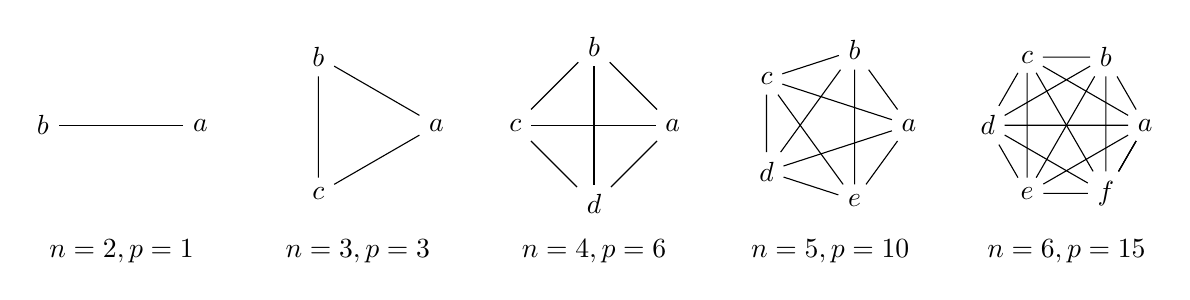
\begin{tikzpicture}[label distance=1.2cm]
\node (2) at (0,0) [label=below:{$n=2, p=1$}]{};
\node (3) at (3,0) [label=below:{$n=3, p=3$}]{};
\node (4) at (6,0) [label=below:{$n=4, p=6$}]{};
\node (5) at (9,0) [label=below:{$n=5, p=10$}]{};
\node (6) at (12,0)[label=below:{$n=6, p=15$}]{};
\path (2) ++(0:1)   node (a) {$a$};
\path (2) ++(180:1) node (b) {$b$};
\draw (a) -- (b);
\path (3) ++(0:1)   node (a) {$a$};
\path (3) ++(120:1) node (b) {$b$};
\path (3) ++(240:1) node (c) {$c$};
\draw (a) -- (b) -- (c) -- (a);
\path (4) ++(0:1)   node (a) {$a$};
\path (4) ++(90:1)  node (b) {$b$};
\path (4) ++(180:1) node (c) {$c$};
\path (4) ++(270:1) node (d) {$d$};
\draw (a) -- (b) -- (c) -- (d) -- (a) ;
\draw (a) -- (c)    (d) -- (b) ;
\path (5) ++(0:1)   node (a) {$a$};
\path (5) ++(72:1)  node (b) {$b$};
\path (5) ++(144:1) node (c) {$c$};
\path (5) ++(216:1) node (d) {$d$};
\path (5) ++(288:1) node (e) {$e$};
\draw (a) -- (b) -- (c) -- (d) -- (e) -- (a) ;
\draw (a) -- (c)    (d) -- (b)    (a) -- (d) ;
\draw (e) -- (b)    (e) -- (c) ;
\path (6) ++(0:1)   node (a) {$a$};
\path (6) ++(60:1)  node (b) {$b$};
\path (6) ++(120:1) node (c) {$c$};
\path (6) ++(180:1) node (d) {$d$};
\path (6) ++(240:1) node (e) {$e$};
\path (6) ++(300:1) node (f) {$f$};
\draw (a) -- (b) -- (c) -- (d) -- (e) -- (f) -- (a) ;
\draw (a) -- (c)    (d) -- (b)    (a) -- (d) ;
\draw (e) -- (b)    (e) -- (c)    (a) -- (f) ;
\draw (d) -- (f)    (b) -- (f)    (a) -- (f) ;
\draw (c) -- (f)    (a) -- (e) ;
\end{tikzpicture}

The basic idea  behind the $t$ test is to divide the difference between 
two values by a measure of how much uncertainty there is about the size 
of that difference. The measure of uncertainty used is the 
\emph{standard error}.

\[
	t=\frac{\textrm{difference between values}}{\textrm{standard error}}
\]

When there is no difference between the values $t$ will be zero, but 
with big differences and/or small errors, will be larger. The $t$ 
distribution below shows how commonly different values of $t$ are found 
under the null hypothesis. 
\begin{center}
\includegraphics[width=0.7\textwidth]{tvals.pdf} 
\end{center}
 
Some points about the plot above:
\begin{compactitem}
	\item The  null hypothesis is that there is no difference between the 
	values but because we only estimate the values from samples, 
	differences will creep in by chance.
	\item Mostly these differences will be small --- hence the peak in 
	the middle --- but sometimes the differences will be large and the 
	errors will be small.
	\item 95\% of the area under the curves are between these two sets of 
	vertical lines. Values of $t$ more extreme than this will only occur 
	1 in 20 times or with a probability ($p$) of 0.05.
	\item The means of small samples are more easily influenced by 
	extreme values and so produce extreme $t$ values more frequently. 
	This is why the red curve above for smaller samples is more flattened 
	out and why the 95\% limits are more spread out.
\end{compactitem}

\section{One sample $t$ tests}

In the simplest example, a $t$ test can be used to test whether the 
mean of a sample is different from a specific value. For example:

\begin{compactitem}
	\item Is the ozone in a set of air samples above the legal limit?
	\item Is the change in a set of patient' weights different from zero?
	\item Is the mean genome size for Odonata smaller than 1.25 pg, which 
	is the average for insects 
	\href{http://www.genomesize.com/statistics.php?stats=insects}{[see 
	here]}?
\end{compactitem}

Oh look! We can test that last one\ldots 

To calculate $t$, we need that observed difference and then the 
standard error of the difference between the mean of our sample and the 
known value. This is calculated using the \emph{variance} and the 
\emph{sample size} ($n$) of the sample ($s$). 

\[se_s = \sqrt{\frac{\textrm{var}(s)}{n}}\]

This simple equation trades off variance --- high variance in the data 
gives higher uncertainty about the location of the mean --- and sample 
size -- more data gives more certainty. So, \emph{low variance} and 
\emph{large datasets} have \emph{small} standard errors; \emph{high 
variance} and \emph{small datasets} have \emph{large} standard errors. 
Variance is calculated using sums of squares and so the square root is 
needed to give a standard error in the same units as the mean.  

So, all we need are three values calculated from the data: mean, 
variance and the number of data points and we can calculate $t$. R can 
do this for us:

\begin{lstlisting}
# calculate the three values from the data:
> mean.gs <- mean(genome$GenomeSize)
> print(mean.gs)
[1] 1.014
> var.gs <- var(genome$GenomeSize)
> print(var.gs)
[1] 0.1397
> n.gs <- length(genome$GenomeSize)
> print(n.gs)
[1] 100
# get the difference
> diff <- mean.gs - 1.25
> print(diff)
[1] -0.2357
# get the standard error
> se.gs <- sqrt(var.gs/n.gs)
> print(se.gs)
[1] 0.03738
# get the t value
> t.gs <- diff/se.gs
> print(t.gs)
[1] -6.306
\end{lstlisting}

\begin{compactitem}[$\quad\star$]
\item Copy and paste the code above into your script in R and run it. 
Read through the code and make sure you understand the steps.
\end{compactitem}

This is a big $t$ value --- values this extreme don't even appear on 
the graph above --- so we would conclude that the mean genome size for 
Odonata is different from the average for insects.

We can do this more easily and get some more information using the 
function {\tt t.test}. The null hypothesis can be set using the option 
(sometimes called a function \emph{argument}) {\tt mu} --- the Greek 
letter $\mu$ is often used to refer to a mean:

\begin{lstlisting}
> t.test(genome$GenomeSize, mu = 1.25)
 
	One Sample t-test
 
 data:  genome$GenomeSize 
 t = -6.306, df = 99, p-value = 8.034e-09
 alternative hypothesis: true mean is not equal to 1.25 
 95 percent confidence interval:
  0.9401 1.0885 
 sample estimates:
 mean of x 
     1.014 
\end{lstlisting}

This confirms the values we calculated by hand and adds a $p$ value. 
The output also gives the degrees of freedom. This is something we will 
come back to later, but the degrees of freedom are basically the number 
of data points minus the number of estimated parameters, which in this 
case is one mean.

The output also gives a confidence interval for the observed mean. 
The mean is the best estimate of the population mean given our sample 
of species of Odonata, but the actual mean for the order could be 
bigger or smaller. The confidence interval tells us the region in which 
we are 95\% confident that this actual mean lies.
 
It is calculated using the $t$ distribution. Remember that $t$ is a 
difference divided by a standard error; if we multiply $t$ by a 
standard error, we get back to a difference. If we pick a pair of $t$ 
values that contain the middle 95\% of the $t$ distribution, as in the 
plot on page 2, then we can multiply that by the standard error from 
the data to get a range above and below the mean.  If we sampled lots 
of sets of 100 species of Odonata, we expect 95\% of the observed means 
to lie inside this range. The code below shows the calculation of the 
confidence interval for the test above.

\begin{lstlisting}
# Find the edges of the middle 95% of a t distribution with 99 df
# (quantiles of the t distribution, so qt)
> tlim <- qt(c(0.025,0.975), df = 99)
> print(tlim)
[1] -1.984 1.984
# use the mean and standard error from above to get a confidence interval
> mean.gs + tlim * se.gs
[1] 0.9401 1.0885
\end{lstlisting}

\begin{compactitem}[$\quad\star$]

	\item Using the {\tt t.test} code above as an template, test whether 
	the body weight (in grams) of Odonata is different from the 
	average\footnote{This slightly dodgy estimate comes from an estimated 
	average volume for arthropods of of 45.21 mm$^3$ and assuming a 
	density of 1 gm per cm$^3$. The volume is from: Orme, C. D. L., 
	Quicke, D. L. J., Cook, J. M. and Purvis, A. (2002), Body size does 
	not predict species richness among the metazoan phyla. Journal of 
	Evolutionary Biology, 15: 235--247.} for arthropods of 0.045 grams.

\end{compactitem}	

\section{Two sample $t$ tests}

It is more common to use a $t$ test to compare the means of two 
samples. This includes questions like:

\begin{compactitem}
	\item Do two rivers have the same concentration of a pollutant?
	\item Do chemical A and chemical B cause different rates of mutation?
	\item Do damselflies and dragonflies have different genome sizes?
\end{compactitem}

The main difference here is that with a one sample $t$ test, we assume 
that one of the means is known exactly: the only error is in the single 
sample. With a two sample test, we are comparing two means estimated 
from samples and both contain error. The graph below illustrates this:
\begin{center}
\includegraphics[width=0.9\textwidth]{twosampleIllustration.pdf} 
\end{center}
	
The vertical lines show the mean (solid lines) and one standard error 
to each side (dashed lines). The red mean is the same in both cases, 
but the second graph shows that this is also estimated from a sample 
with error: the difference in the means looks less convincing and we'd 
expect a smaller $t$ value. The $t$ tests in for these two graphs 
confirm this:

\begin{compactitem}
\item The mean for blue is significantly different from 16.74 
(mean=14.98, se=0.38, df=59, $t$=-4.65, $p$=0.00002). 
\item The means of blue and red are significantly different (blue: 
mean=14.98, se=0.38; red: mean=16.74, se=0.42; df=118, $t$=-3.13, 
$p$=0.002)
\end{compactitem}

\begin{compactitem}[$\quad\star$]
\item Have a close look at the previous two statements. This shows the 
kind of detail needed when reporting the results of $t$ tests. The 
following is \emph{not} acceptable: The means of blue and red are 
significantly different ($p=0.002$).
\end{compactitem}

So, with two samples, we shouldn't be so confident about the difference 
between the values --- it should have a higher standard error. We can 
do this simply by combining the variance and sample size for the two 
samples ($a$ and $b$) into the calculation:

\[
se_{a-b}= \sqrt{\frac{\textrm{var}(a)}{n_a} + \frac{\textrm{var}(b)}{n_b}}
\]

We'll use a $t$ test to address that last question: are the genome 
sizes of Anisoptera and Zygoptera different? First, we'll do this by 
hand. We'll use a really handy function {\tt tapply(X, INDEX, FUN)} to 
quickly find the values for the two groups: it takes some values (X), 
splits those values into groups based on a factor (INDEX) and runs each 
group through another function (FUN). 

\begin{lstlisting}
# calculate the three values from the data
> mean.gs <- tapply(X = genome$GenomeSize, INDEX = genome$Suborder, FUN = mean)
> print(mean.gs)
Anisoptera 	Zygoptera
1.018				1.012
> var.gs <- tapply(X = genome$GenomeSize, INDEX = genome$Suborder, FUN = var)
> print(var.gs)
Anisoptera 	Zygoptera
0.18458 		0.06946
> n.gs <- tapply(X = genome$GenomeSize, INDEX = genome$Suborder, FUN = length)
> print(n.gs)
Anisoptera 	Zygoptera
38					62

# get the difference
> diff <- mean.gs[1] - mean.gs[2]
> print(diff)
Anisoptera
-0.006647

# get the standard error of the difference
> se.gs <- sqrt((var.gs[1]/n.gs[1]) + (var.gs[2]/n.gs[2]))
> print(se.gs)
Anisoptera
0.06932

# get the t value
> t.gs <- diff/se.gs
> print(t.gs)
Anisoptera

-0.09589

\end{lstlisting}
 
\begin{compactitem}[$\quad\star$]
\item Type the code above into your script in R and run it. Again, read 
through the code and make sure you understand the steps.
\end{compactitem}

The {\tt t.test} function automates this all for us, and we can use a 
formula (see Chapter \ref{ch:ExpDesign}) to get a test between the two 
suborders.

\begin{lstlisting}
>  t.test(GenomeSize ~ Suborder, data = genome)
 
 	Welch Two Sample t-test
 
 data:  GenomeSize by Suborder 
 t = -0.0959, df = 98, p-value = 0.9238
 alternative hypothesis: true difference in means is not equal to 0 
 95 percent confidence interval:
  -0.1442  0.1309 
 sample estimates:
 mean in group Anisoptera  mean in group Zygoptera 
                    1.012                    1.018 
 
\end{lstlisting}
 
The output looks very similar to the one sample test, except that the 
output  now gives two estimated means, rather than one and it reports 
the $p$ value for the calculated $t$ value.

\begin{compactitem}[$\quad\star$]
\item Add this to your script and run it.
\item Copy and modify this in your script to test whether the body 
weight of the two suborders are different.
\end{compactitem}

\section{$F$ tests for equal variance}

$F$ tests are used to compare the variances of two samples or 
populations. You will most prominently see them in analysis of variance 
(ANOVA), to test the hypothesis that the means of a given set of 
normally distributed populations all have the same variance. 

Let's use our genomesize datast to have a look at F-tests as well. 
Ideally, the $t$ test should be used with data that are: i) 
\emph{relatively normally distributed}, so that means can be estimated 
sensibly; and ii) have \emph{similar variances}. We'll deal with the 
similar variance question here using an $F$ test for equal variances. 

First, let's visualize the data. As I hope you've already noticed, this 
session has been neglecting one very important part of analysis --- 
\emph{plotting the data}. We are going to compare two plots, so it 
helps to have them side by side in the same window. We can use the 
function {\tt par} to change a set of options called graphics 
parameters to get R to do this. The option to change is {\tt mfrow}. 
This sets a graphics window to include \emph{m}ultiple \emph{f}igures 
and we need to tell R the number of rows and columns to divide the 
window into: {\tt par(mfrow=c(1,2))}.
  
\begin{compactitem}[$\quad\star$]
\item Copy {\tt par(mfrow=c(1,2))} into your script, add a comment and 
run it.
\item Using your (rapidly improving!) R skills, create a boxplot comparing the 
genome sizes of the two suborders.
\item Add another boxplot beside it comparing the body weight of the 
two suborders.
\end{compactitem}
It should look like this:
\begin{center}
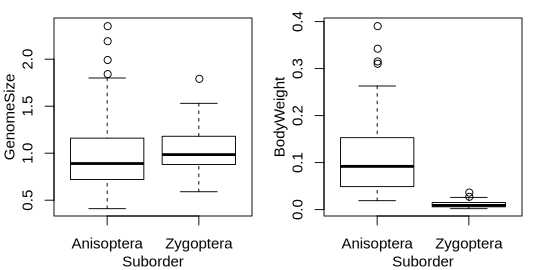
\includegraphics[width=0.9\textwidth]{bxp.pdf} 
\end{center}

The distribution of the test statistic $F$ is simply the ratio of the 
variances for sample $a$ and $b$: $\textrm{var}(a)/\textrm{var}(b)$. If 
the two variances are the same then $F=1$; if $\textrm{var}(a) > 
\textrm{var}(b)$ then $F > 1$; and if $\textrm{var}(a) < 
\textrm{var}(b)$ then $F < 1$ (\ref{fig:fdist}).

\begin{figure}
	\centering
	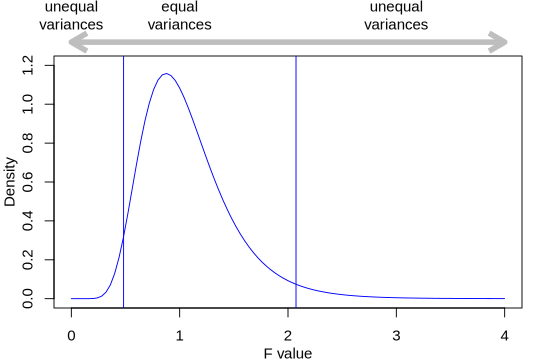
\includegraphics[width=0.7\textwidth]{fvals.pdf} 
	\caption[Caption for LOF]{The F distribution. The two vertical blue 
	lines show the edges of the central 95\% of the area of the curve: if 
	the two samples are drawn at random from a population with the same 
	variance then values of $F < 0.482$ or $> 2.074$ are observed fewer 
	than 1 time in 20 ($p\le0.05$ )\protect\footnotemark . The shape of 
	the $F$ distribution changes depending on the amount of data in each 
	of the two samples but will always be centered 
	near 1 and with a tail to the right (right-skewed). Note that the 
	F-distribution arises as the ratio of two appropriately scaled {\it 
	chi-square distributed variates}, because, as we saw above, variances 
	should be chi-square distributed.}
\label{fig:fdist} 
\end{figure}
\footnote{Note that $1/0.482 \approx 2.074$ 
	and $1/2.074 \approx 0.482$: in this case, it doesn't matter which 
	way round you compare the two variances!}

We can use R to calculate $F$ for the variance in genome size in each 
of the two suborders. We calculated the variance for the $t$ test 
above, so we can just do this:

\begin{lstlisting}
> var.gs[1]/var.gs[2]
Anisoptera
		2.657
\end{lstlisting}

That's quite a big $F$ value and we can use the function {\tt var.test} 
to do all the calculations for us and give us the actual $p$ value:

\begin{lstlisting}
> var.test(GenomeSize ~ Suborder, data = genome) 
 	F test to compare two variances
 
 data:  GenomeSize by Suborder 
 F = 2.657, num df = 61, denom df = 37, p-value = 0.001946
 alternative hypothesis: true ratio of variances is not equal to 1 
 95 percent confidence interval:
  1.449 4.671 
 sample estimates:
 ratio of variances 
              2.657 
\end{lstlisting}

It produces the same value that we calculated by hand and shows that, 
if the two samples are drawn from populations with the same variance,  
an $F$ value this extreme will only be observed roughly 1 time in 500 
($1/0.00195 \approx 500$) .
 
\begin{compactitem}[$\quad\star$]
\item Open a new empty script called {\tt FTests.R}.
\item In this write your script to test whether the variances in the 
body weight of the two suborders from the {\tt GenomSize} dataset are 
different.
\end{compactitem}
 
There are clearly problems with the variance in both examples. The next 
two sections present ways to address these kinds of problems.

\section{$t$ tests revisited}

The first thing to say is that R is aware of the problem with the 
variance. If you look back at the output from the previous $t$ tests, 
you will see that the degrees of freedom vary a lot. We have 100 
observations and -- after subtracting one for each mean we calculate 
--- our degrees of freedom should be either 99 (one sample test) or 98 
(two sample test). What we actually see are smaller numbers, with the 
smallest being {\tt df = 60.503} for the two sample test of body 
weight. 

 
The explanation is that R is applying a \emph{penalty} to the degrees 
of freedom to account for differences in variance. With fewer degrees 
for freedom, more extreme $t$ values are more likely and so it is 
harder to find significant results. This doesn't mean we can forget 
about checking the variances or plotting the data!

In this case, we can also apply a transformation to the data in order 
to make the variances more equal. Forgetting the wings and assuming 
Odonata are shaped like a box, the model in the graph below shows how 
volume changes with length: equal changes in length do not lead to 
equal changes in volume and longer species will have a 
disproportionately large volume. This is a classic feature of 
morphological data known as allometric scaling and we'll look at it 
again in Chapter \ref{ch:ANOVA}. In the meantime, a log transformation will 
turn body weight from a skewed distribution to a more normal 
distribution.
 
\begin{center}
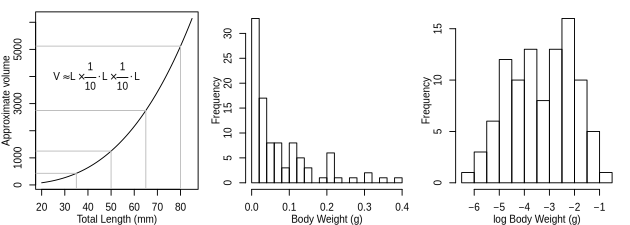
\includegraphics[width=\textwidth]{transform.pdf} 
\end{center}

% We can create a new variable in the {\tt genome} data frame of 
$\log_e$ body weight as follows:

\begin{lstlisting}
> genome$logBodyWeight <- log(genome$BodyWeight)
\end{lstlisting}


\begin{compactitem}[$\quad\star$]
\item Copy the line into your script and run it.
\item Now write three lines of code to get a boxplot of $\log_e$ body 
weight and then run a variance test and $t$ test on the differences in 
$\log_e$ body weight between suborders.
\end{compactitem}

This gives a much clearer result --- the variances are almost identical 
and the differences between the suborders are much more cleanly tested.

 
\section{Non-parametric tests}

What happens if there isn't a convenient transformation for the 
variable that gives roughly constant variation and equal variance?  In 
a parametric test, like the $t$ and $F$ test above, we use parameters 
(mean and variance) to describe the data, assume these describe the 
data well and then just use these parameters to run the test. If these 
assumptions don't seem very sound, the non-parametric tests provide a 
way of using the ranks of the data to test for differences. They aren't 
as powerful --- they are less likely to reveal significant differences 
--- but they are more robust. The most commonly used alternative is the 
Wilcoxon test, which uses the function {\tt wilcox.test} in R.

\begin{compactitem}[$\quad\star$]

\item Using {\tt wilcox.test} as a replacement for {\tt t.test}, repeat 
the one and two sample $t$ test for genome size and body weight.
\item Compare the two results.
\item Repeat the same with the predator and prey body mass data from 
the plotting and visualization chapter in SilBioComp.pdf -- check how 
different the results are when using $t$ vs. Wilcoxon test.

\end{compactitem}
